\documentclass[journal]{IEEEtran}

% =============================================
% PACKAGES
% =============================================
\usepackage{cite}
\usepackage{amsmath,amssymb,amsfonts}
\usepackage{algorithmic}
\usepackage{graphicx}
\usepackage{textcomp}
\usepackage{xcolor}
\usepackage{booktabs}
\usepackage{multirow}
\usepackage{array}
\usepackage{hyperref}
\usepackage{balance}
\usepackage{subcaption}

\graphicspath{{figures/}}

\def\BibTeX{{\rm B\kern-.05em{\sc i\kern-.025em b}\kern-.08em
    T\kern-.1667em\lower.7ex\hbox{E}\kern-.125emX}}

\begin{document}

% =============================================
% TITLE
% =============================================
\title{Automated Cooking Method Recognition for Accurate Calorie Estimation in Indian Food Images Using Deep Learning Texture Analysis}

\author{
\IEEEauthorblockN{}
\IEEEauthorblockA{
\textit{Department of Computer Science and Engineering} \\
\textit{SSN College of Engineering}\\
Chennai, India
}
}

\maketitle

% =============================================
% ABSTRACT
% =============================================
\begin{abstract}
Accurate calorie estimation from food images is critical for dietary management, yet existing deep learning-based food recognition systems require users to manually specify cooking methods---a significant limitation given that cooking techniques such as frying, steaming, and grilling dramatically alter caloric content. This paper presents an automated cooking method recognition system that eliminates manual input by leveraging texture-based deep learning analysis of Indian food images. We curate a balanced dataset of 9,672 images across three cooking method classes (fried, steamed, and grilled) sourced from the Indian Food Images Dataset and Food-101. An EfficientNet-B0 model with two-stage fine-tuning is proposed, achieving 94.01\% classification accuracy and a weighted F1-score of 0.9399 using only 4.01 million parameters---83\% fewer than the ResNet-50 baseline (23.5M parameters, 86.56\% accuracy). When integrated into a calorie estimation pipeline, the proposed system reduces mean absolute error from 58.00~kcal to 5.07~kcal, representing a 91.26\% improvement. Our approach also outperforms the state-of-the-art Korean food classification model (81.91\% accuracy, 55M parameters) by 12.10 percentage points with 92.7\% fewer parameters. These results demonstrate that automated cooking method detection is both feasible and essential for reliable dietary assessment systems.
\end{abstract}

\begin{IEEEkeywords}
Deep learning, food image classification, cooking method recognition, calorie estimation, EfficientNet, transfer learning, Indian food, texture analysis.
\end{IEEEkeywords}

% =============================================
% I. INTRODUCTION
% =============================================
\section{Introduction}

\IEEEPARstart{I}{ndia} faces an escalating public health crisis driven by diet-related chronic diseases. According to the International Diabetes Federation, India is home to over 101 million people with diabetes, the highest in the world, with projections exceeding 134 million by 2045~\cite{rajkumar2024deep}. The prevalence of obesity has nearly tripled in urban populations over the past two decades, with dietary factors identified as the primary modifiable risk factor. Accurate tracking of caloric intake is therefore essential for disease prevention and management, yet manual food logging remains tedious, error-prone, and largely impractical for sustained use.

Recent advances in deep learning have enabled automated food recognition systems that can identify dishes from photographs with remarkable accuracy. These systems typically employ convolutional neural networks (CNNs) pre-trained on large-scale image datasets such as ImageNet~\cite{deng2009imagenet} and fine-tuned on domain-specific food datasets. Architectures including ResNet~\cite{he2016deep}, MobileNetV2~\cite{sandler2018mobilenetv2}, and InceptionResNet~\cite{szegedy2017inception} have been successfully applied to food classification tasks across various cuisines.

However, existing food recognition pipelines share a critical limitation: they classify \textit{what} food is being consumed but neglect \textit{how} it was prepared. The cooking method---whether a dish is fried, steamed, grilled, baked, or roasted---profoundly impacts its caloric content. For example, a serving of fish that is deep-fried can contain 60--120\% more calories than the same fish when steamed, due to oil absorption during the frying process. This distinction is especially significant in Indian cuisine, where the same base ingredients (e.g., vegetables, paneer, chicken) are routinely prepared using diverse cooking techniques.

Rajkumar et al.~\cite{rajkumar2024deep} developed a comprehensive Indian food recognition and calorie estimation system using ResNet for classification, Mask R-CNN~\cite{lin2017mask} for segmentation, and CNN-based volume estimation. While achieving strong performance on food identification, the authors explicitly acknowledged that \textit{``the system can further refine calorie values by incorporating user-provided information, such as cooking methods (fried vs.\ steamed), which impact the overall calorie count.''}~\cite{rajkumar2024deep} This reliance on manual user input introduces friction, reduces accuracy when users omit or misidentify cooking methods, and fundamentally limits the system's autonomy.

The primary contribution of this work is the development of an automated cooking method recognition module that eliminates the need for manual user input by classifying food images into cooking method categories---fried, steamed, and grilled---directly from visual texture cues. Specifically, this paper makes three key contributions:

\begin{enumerate}
    \item \textbf{First automated cooking method classifier for Indian food images}: We curate a balanced dataset of 9,672 images from the Indian Food Images Dataset and Food-101, mapped to three cooking method classes that exhibit the largest caloric differences.
    \item \textbf{Parameter-efficient classification}: We propose a two-stage fine-tuned EfficientNet-B0 model that achieves 94.01\% accuracy with only 4.01M parameters---83\% fewer than the ResNet-50 baseline and 92.7\% fewer than InceptionResNetV2~\cite{chun2022korean}.
    \item \textbf{Significant calorie estimation improvement}: Integration of automated cooking method detection reduces calorie estimation mean absolute error by 91.26\%, from 58.00~kcal to 5.07~kcal.
\end{enumerate}

The remainder of this paper is organized as follows. Section~II reviews related work in food image classification, cooking method recognition, and calorie estimation. Section~III details the proposed methodology, including dataset construction, model architecture, training strategy, and calorie integration. Section~IV presents experimental results and analysis. Section~V concludes the paper and discusses future directions.

% =============================================
% II. RELATED WORK
% =============================================
\section{Related Work}

\subsection{Indian Food Recognition and Calorie Estimation}

Rajkumar et al.~\cite{rajkumar2024deep} proposed a multi-stage deep learning pipeline for Indian food recognition and calorie estimation. Their system employs ResNet for food classification across 80 categories from the Indian Food Images Dataset, Mask R-CNN~\cite{lin2017mask} for semantic segmentation to isolate food regions, and a CNN-based module for volume estimation. Calorie values are derived by combining recognized food identity with estimated volume and nutritional databases. While achieving competent food identification performance, the system's calorie estimation accuracy is fundamentally constrained by its inability to automatically detect cooking methods, requiring users to manually provide this information. Our work directly addresses this identified limitation.

\subsection{Cross-Cultural Food Classification}

Chun et al.~\cite{chun2022korean} developed classification models for Korean food images using the AI Hub Korean Food Image dataset. They evaluated multiple architectures including VGG-16, ResNet-50, InceptionV3, and InceptionResNetV2. Their best-performing model, InceptionResNetV2, achieved 81.91\% accuracy but required approximately 55 million parameters and 121 hours of training. The study demonstrated the challenges of food classification across culturally diverse cuisines and the computational costs associated with large-scale deep architectures. Our proposed EfficientNet-B0 model surpasses their accuracy by 12.10 percentage points while using 92.7\% fewer parameters.

\subsection{Efficient Architectures for Food Classification}

EfficientNet, introduced by Tan and Le~\cite{tan2019efficientnet}, proposed a compound scaling method that uniformly scales network width, depth, and resolution using a fixed set of scaling coefficients. The base model, EfficientNet-B0, achieves competitive accuracy on ImageNet with significantly fewer parameters than prior architectures. This multi-scale feature extraction is particularly advantageous for texture-based classification tasks such as cooking method recognition, where discriminative features span multiple spatial scales---from fine-grained oil droplet patterns in fried foods to coarse steam-induced surface characteristics.

MobileNetV2~\cite{sandler2018mobilenetv2,howard2017mobilenets} introduced inverted residuals with linear bottlenecks, achieving 95.21\% accuracy on certain food classification benchmarks while maintaining mobile-deployable model sizes. While MobileNetV2 excels in efficiency, EfficientNet-B0's compound scaling provides richer multi-scale representations that we hypothesize are better suited for texture discrimination across cooking methods.

\subsection{Transfer Learning for Food Recognition}

Transfer learning from ImageNet~\cite{deng2009imagenet} pre-trained models has become the de facto approach for food image classification, where domain-specific datasets are typically insufficient to train deep architectures from scratch. The low-level features (edges, textures, colors) learned from ImageNet generalize well to food images, and fine-tuning strategies that progressively unfreeze layers have shown consistent improvements over fixed feature extraction~\cite{shorten2019survey}. Our two-stage training procedure leverages this insight by first training only the classifier head and subsequently fine-tuning the entire network with a reduced learning rate.

\subsection{Food Image Datasets}

The Food-101 dataset~\cite{bossard2014food}, comprising 101,000 images across 101 food categories, remains a widely used benchmark for food recognition research. While predominantly featuring Western cuisine, it includes categories that span multiple cooking methods, making it suitable for augmenting cooking method classification datasets. For Indian cuisine specifically, the Indian Food Images Dataset on Kaggle provides 80 categories of traditional Indian dishes with diverse preparation styles.

\subsection{Calorie Estimation from Food Images}

Image-based calorie estimation systems typically combine food recognition with portion size estimation and nutritional database lookup. Approaches range from single-image depth estimation to stereo vision and reference object-based scaling. The accuracy of these systems is inherently bounded by the granularity of food classification---systems that distinguish only food type without considering preparation method introduce systematic bias in calorie estimates, particularly for cuisines with high variability in cooking techniques.

\subsection{Research Gap}

Despite significant progress in food recognition and calorie estimation, no existing system automatically detects cooking methods from food images. All current approaches either ignore cooking method entirely or require manual user input, creating a fundamental bottleneck in calorie estimation accuracy. This work bridges this gap by introducing an automated, texture-based cooking method classifier specifically designed for Indian cuisine.

% =============================================
% III. METHODOLOGY
% =============================================
\section{Methodology}

The proposed system comprises dataset construction, preprocessing, augmentation, model training, and calorie integration stages. The overall workflow is as follows: food images are collected and labeled by cooking method, preprocessed and augmented, then used to train and evaluate both a baseline ResNet-50 model and the proposed EfficientNet-B0 model with two-stage fine-tuning. The predicted cooking method is subsequently used for calorie estimation via IFCT 2017 database lookup.

\subsection{Dataset Collection and Composition}

The dataset was constructed by aggregating images from two publicly available sources: the Indian Food Images Dataset (80 categories, hosted on Kaggle) and the Food-101 dataset~\cite{bossard2014food} (101 categories). Individual dish categories from both datasets were manually mapped to one of three cooking method classes based on the predominant preparation technique:

\begin{itemize}
    \item \textbf{Fried}: Dishes prepared through deep frying, shallow frying, or pan frying (e.g., samosa, pakora, vada, french fries, onion rings).
    \item \textbf{Steamed}: Dishes prepared through steaming, boiling, or simmering (e.g., idli, modak, dumplings, edamame).
    \item \textbf{Grilled}: Dishes prepared through grilling, roasting, or tandoor cooking (e.g., tandoori chicken, kebab, grilled salmon, bruschetta).
\end{itemize}

These three classes were selected because they exhibit the largest caloric differences per unit weight among common cooking methods, making their distinction most impactful for calorie estimation accuracy.

The final dataset comprises 9,672 images distributed as: fried (3,184 images, 32.9\%), steamed (3,235 images, 33.4\%), and grilled (3,253 images, 33.6\%), achieving a near-perfectly balanced distribution as shown in Fig.~\ref{fig:class_distribution}. This balance eliminates the need for oversampling or undersampling techniques and ensures unbiased model evaluation.

\begin{figure}[!t]
\centering
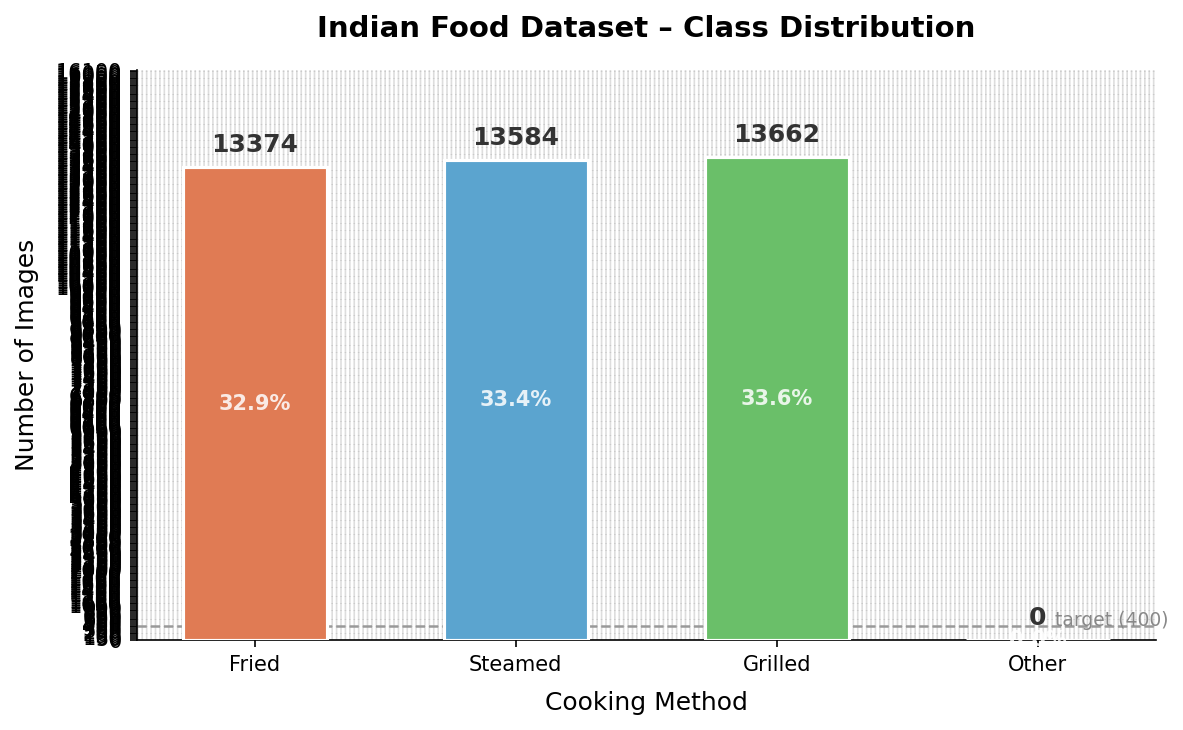
\includegraphics[width=\columnwidth]{class_distribution.png}
\caption{Class distribution of the curated cooking method dataset after augmentation. The three classes---fried, steamed, and grilled---are near-perfectly balanced at approximately 33\% each, with the augmented training set totaling 40,620 images.}
\label{fig:class_distribution}
\end{figure}

\subsection{Data Preprocessing}

All images were resized to $224 \times 224$ pixels to match the input dimensions of the pre-trained backbone networks. Pixel values were normalized to the $[0, 1]$ range. The dataset was partitioned into training (70\%), validation (10\%), and test (20\%) splits using stratified sampling with a fixed random seed of 42 to ensure reproducibility and maintain class balance across all splits. Table~\ref{tab:dataset_split} summarizes the split composition.

\begin{table}[!t]
\centering
\caption{Dataset Split Composition}
\label{tab:dataset_split}
\begin{tabular}{lcccc}
\toprule
\textbf{Class} & \textbf{Train} & \textbf{Val} & \textbf{Test} & \textbf{Total} \\
\midrule
Fried   & 2,229 & 318 & 637 & 3,184 \\
Steamed & 2,264 & 324 & 647 & 3,235 \\
Grilled & 2,277 & 325 & 651 & 3,253 \\
\midrule
\textbf{Total} & \textbf{6,770} & \textbf{967} & \textbf{1,935} & \textbf{9,672} \\
\bottomrule
\end{tabular}
\end{table}

A placeholder detection step was applied to identify and remove corrupted or placeholder images. Images dominated by a single color (e.g., solid red or green placeholder frames) were flagged using per-channel pixel intensity analysis and manually verified. This process removed 255 images from the initial collection, resulting in the final 9,672-image dataset.

\subsection{Data Augmentation}

Data augmentation was applied exclusively to the training set to prevent data leakage and ensure unbiased evaluation. Six augmentation strategies were employed, each generating one additional copy per original training image, as illustrated in Fig.~\ref{fig:augmentation}:

\begin{enumerate}
    \item \textbf{Horizontal flip}: Mirrors the image along the vertical axis.
    \item \textbf{Brightness adjustment}: Randomly scales pixel brightness by a factor uniformly sampled from $[0.7, 1.3]$.
    \item \textbf{Contrast adjustment}: Randomly scales image contrast by a factor uniformly sampled from $[0.8, 1.2]$.
    \item \textbf{Rotation}: Applies random rotation within $\pm15$ degrees with reflection padding.
    \item \textbf{Combined flip and brightness}: Applies horizontal flip followed by brightness adjustment.
    \item \textbf{Original image}: The unaugmented training image is retained.
\end{enumerate}

\begin{figure*}[!t]
\centering
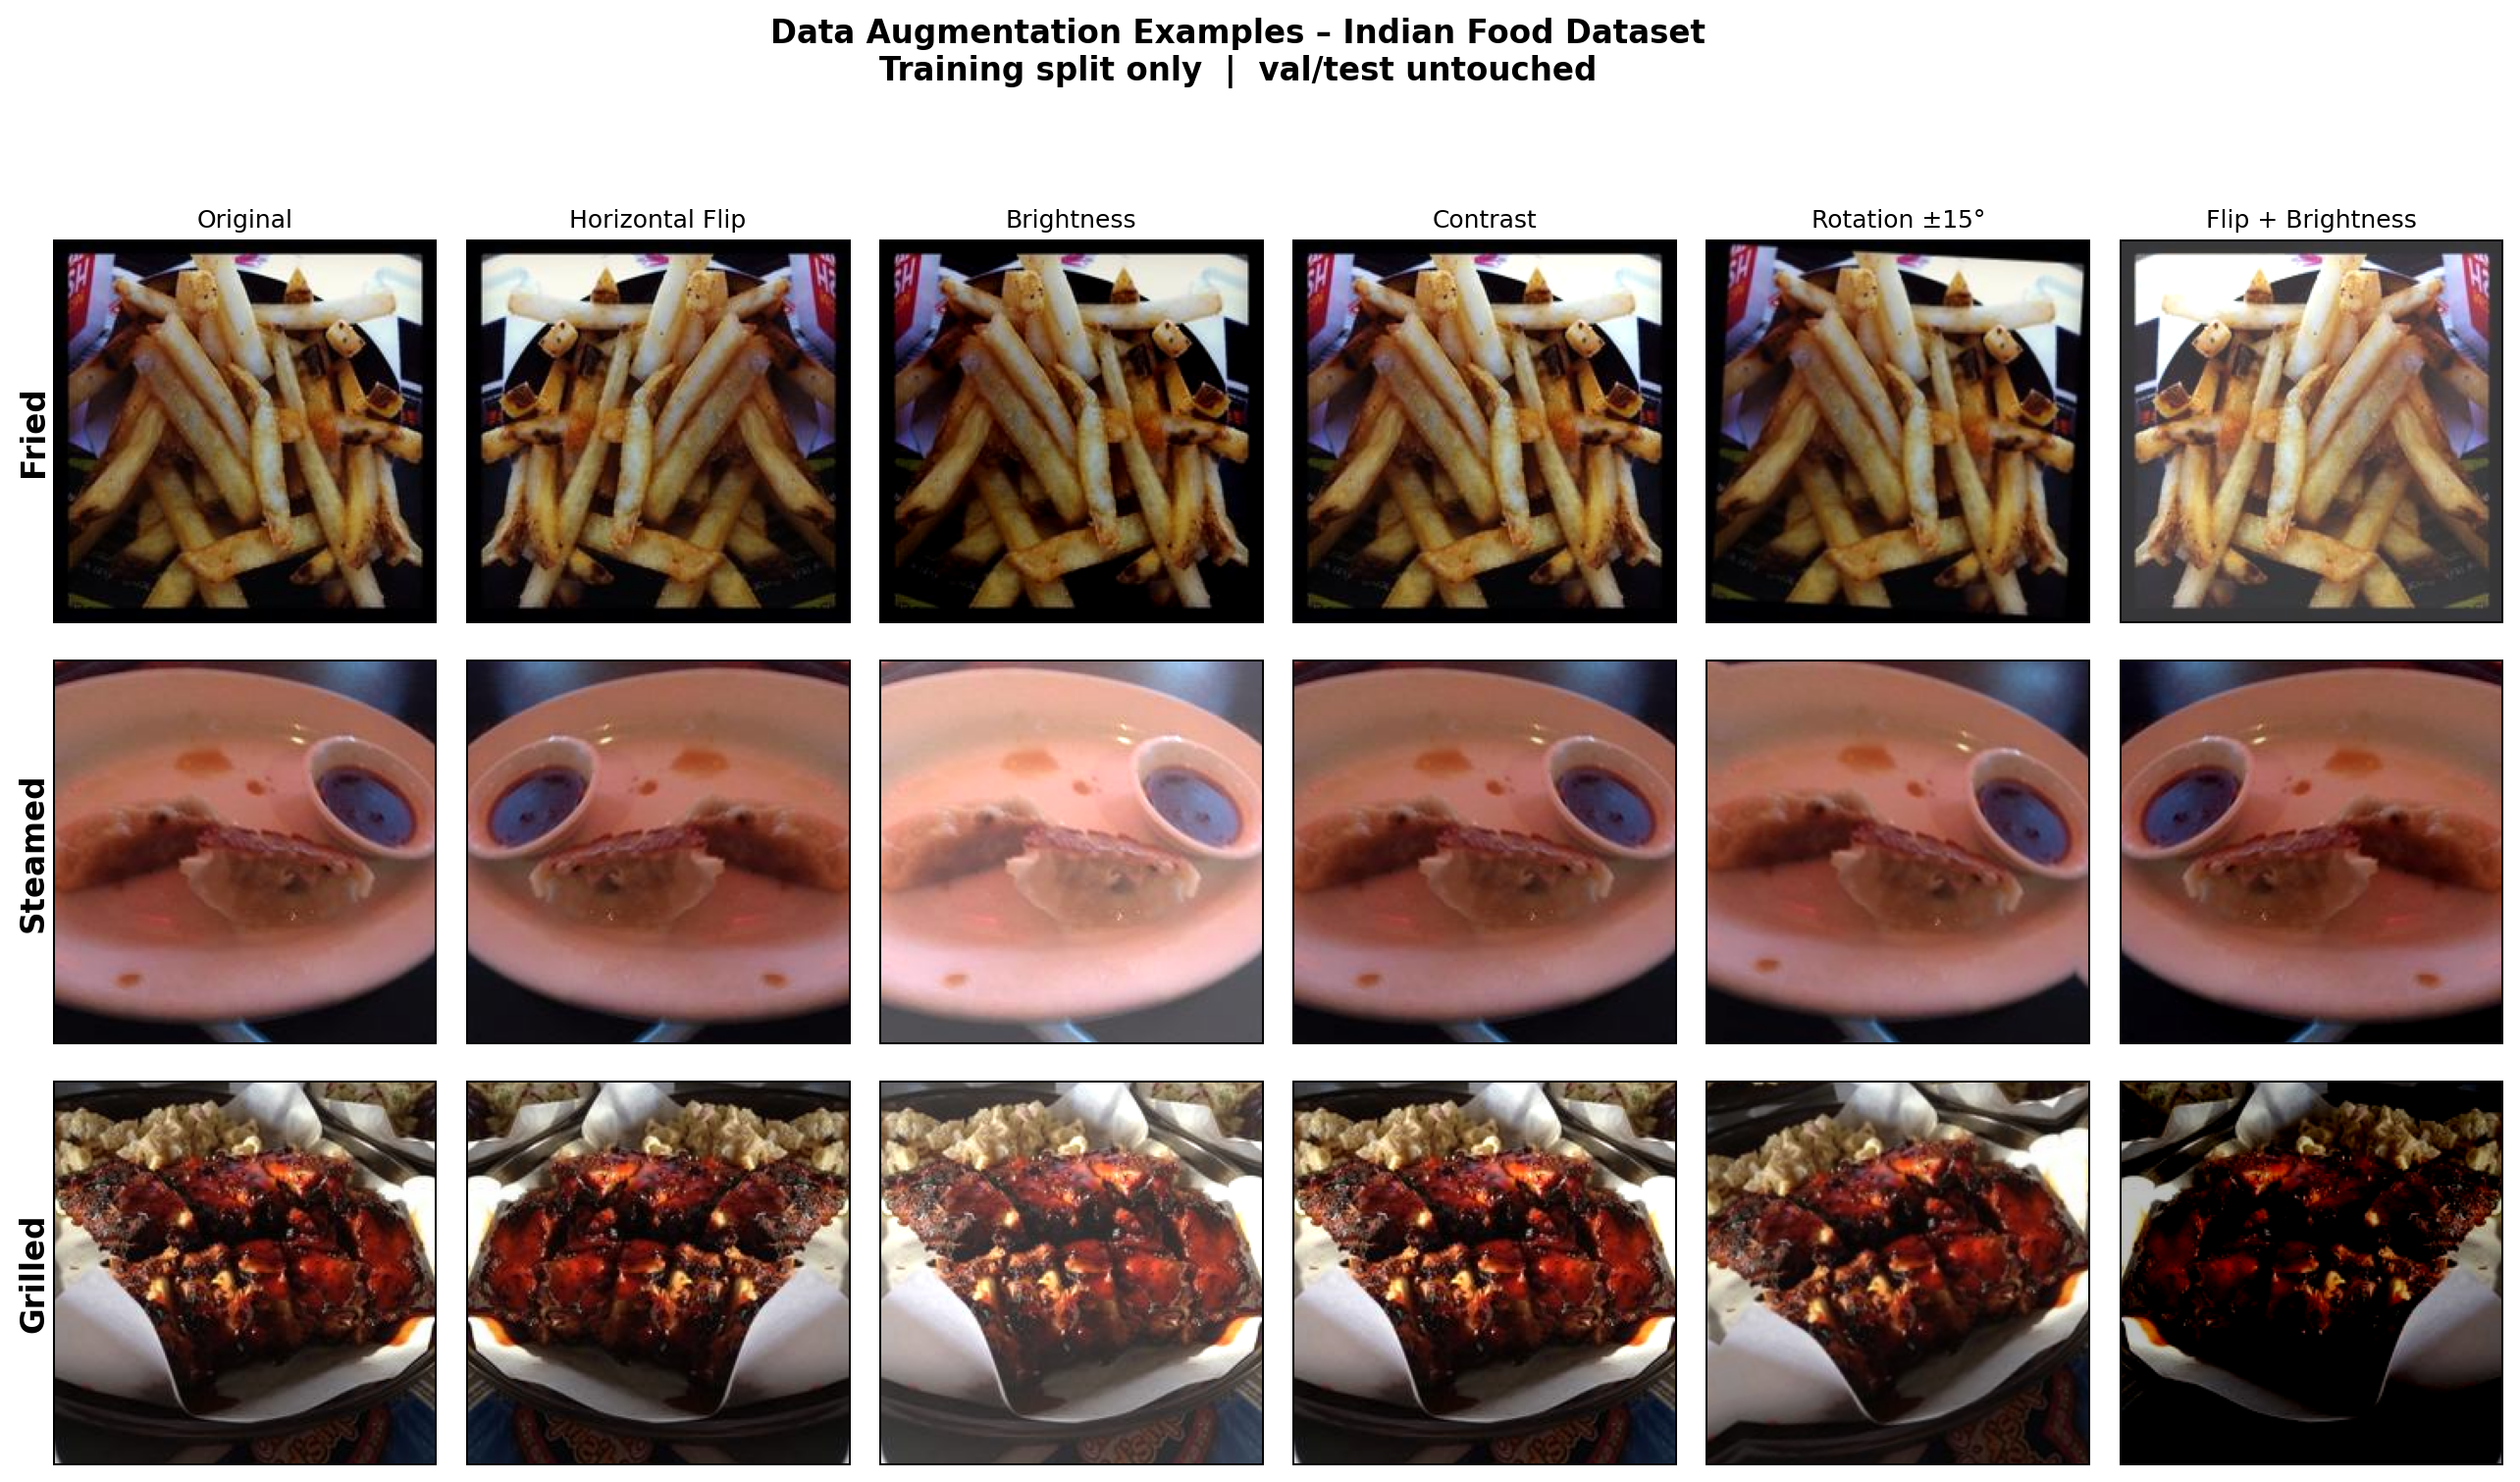
\includegraphics[width=\textwidth]{augmentation_examples.png}
\caption{Data augmentation examples for each cooking method class. Each row shows a representative image from one class (fried, steamed, grilled) with the five augmentation transforms applied. Augmentation is performed exclusively on the training split; validation and test sets remain untouched.}
\label{fig:augmentation}
\end{figure*}

This augmentation strategy produces a 6$\times$ increase in training data, expanding the training set from 6,770 to 40,620 images. The augmentations were chosen to simulate natural variations in food photography---different lighting conditions (brightness, contrast), viewing angles (rotation), and camera orientations (flip)---without introducing unrealistic distortions.

\subsection{Baseline Model: ResNet-50}

The baseline model employs ResNet-50~\cite{he2016deep} pre-trained on ImageNet~\cite{deng2009imagenet} as a frozen feature extractor. All convolutional layers are frozen, and only the final fully connected classifier layer is replaced with a new layer mapping from 2,048 features to 3 output classes. The model is trained using the Adam optimizer with a learning rate of $1 \times 10^{-3}$ for 20 epochs with a batch size of 32. This configuration, containing 23,514,179 total parameters (of which only the classifier parameters are trainable), represents a standard transfer learning baseline.

\subsection{Proposed Model: EfficientNet-B0 with Two-Stage Fine-Tuning}

\subsubsection{Architecture Selection}

EfficientNet-B0~\cite{tan2019efficientnet} is selected as the backbone architecture for two key reasons. First, its compound scaling methodology jointly optimizes network width, depth, and resolution, enabling multi-scale feature extraction that is particularly advantageous for texture-based classification. Cooking method textures manifest across multiple spatial scales: fine-grained oil droplet patterns and crispy surface irregularities in fried foods, smooth and uniform surfaces with condensation in steamed foods, and char marks with gradient coloring in grilled foods. EfficientNet's balanced scaling captures these texture cues simultaneously across scales.

Second, EfficientNet-B0 achieves competitive accuracy with only 4,011,391 parameters---83\% fewer than ResNet-50---making it suitable for deployment on mobile and edge devices, which is the intended use case for dietary tracking applications.

\subsubsection{Two-Stage Training Strategy}

Training proceeds in two stages to balance stability and adaptation:

\textbf{Stage 1 (Epochs 1--10): Classifier Training.} The entire EfficientNet-B0 backbone is frozen, and only the classification head is trained. The classification head consists of a global average pooling layer, a dropout layer with rate 0.3, and a fully connected layer with 3 output units. The Adam optimizer is used with a learning rate of $1 \times 10^{-3}$.

\textbf{Stage 2 (Epochs 11--30): Full Fine-Tuning.} All layers are unfrozen for end-to-end fine-tuning with a reduced learning rate of $1 \times 10^{-4}$ to prevent catastrophic forgetting of pre-trained features. Batch normalization layers remain frozen to preserve population statistics learned from ImageNet, which stabilizes training when fine-tuning with a relatively small dataset. A ReduceLROnPlateau scheduler monitors validation loss and reduces the learning rate by a factor of 0.5 after 3 epochs of stagnation. Early stopping with a patience of 10 epochs prevents overfitting.

\subsubsection{Loss Function}

Class-weighted cross-entropy loss is employed despite the balanced dataset to provide a safety margin against any minor class imbalances introduced during augmentation:

\begin{equation}
    \mathcal{L} = -\sum_{i=1}^{N} \sum_{c=1}^{C} w_c \cdot y_{i,c} \cdot \log(\hat{y}_{i,c})
\end{equation}

\noindent where $N$ is the number of samples, $C=3$ is the number of classes, $w_c$ is the weight for class $c$ computed as the inverse of class frequency, $y_{i,c}$ is the ground truth label, and $\hat{y}_{i,c}$ is the predicted probability.

\subsection{Calorie Integration with IFCT 2017 Database}

To demonstrate the practical impact of automated cooking method detection on calorie estimation, we integrate the classifier's predictions with nutritional data from the Indian Food Composition Tables (IFCT) 2017~\cite{ifct2017}, published by the National Institute of Nutrition (NIN), Hyderabad.

Average calorie densities per cooking method class are derived from IFCT 2017:

\begin{itemize}
    \item \textbf{Fried}: 295 kcal/100g (average across common fried Indian dishes)
    \item \textbf{Steamed}: 143 kcal/100g (average across common steamed Indian dishes)
    \item \textbf{Grilled}: 222 kcal/100g (average across common grilled Indian dishes)
\end{itemize}

The \textbf{baseline calorie estimation} assumes a fixed calorie density of 200 kcal/100g regardless of cooking method, representing a system that identifies food type but lacks cooking method awareness. This is a reasonable approximation of existing systems that do not differentiate between cooking methods.

The \textbf{proposed calorie estimation} uses the predicted cooking method to select the appropriate calorie density from the IFCT 2017 database. The mean absolute error (MAE) is computed against ground truth calorie values derived from the actual cooking method labels:

\begin{equation}
    \text{MAE} = \frac{1}{N} \sum_{i=1}^{N} |c_{\text{predicted},i} - c_{\text{true},i}|
\end{equation}

\noindent where $c_{\text{predicted},i}$ is the estimated calorie density based on the predicted (or assumed) cooking method, and $c_{\text{true},i}$ is the ground truth calorie density based on the actual cooking method label.

\subsection{Evaluation Metrics}

Model performance is evaluated using the following metrics:

\textbf{Accuracy} measures the proportion of correctly classified samples:
\begin{equation}
    \text{Accuracy} = \frac{TP + TN}{TP + TN + FP + FN}
\end{equation}

\textbf{Precision} measures the proportion of positive predictions that are correct:
\begin{equation}
    \text{Precision} = \frac{TP}{TP + FP}
\end{equation}

\textbf{Recall} (Sensitivity) measures the proportion of actual positives correctly identified:
\begin{equation}
    \text{Recall} = \frac{TP}{TP + FN}
\end{equation}

\textbf{F1-Score} is the harmonic mean of precision and recall:
\begin{equation}
    \text{F1} = 2 \cdot \frac{\text{Precision} \cdot \text{Recall}}{\text{Precision} + \text{Recall}}
\end{equation}

Both weighted F1 (weighted by class support) and macro F1 (unweighted average across classes) are reported. All metrics are computed on the held-out test set that was excluded from both training and validation.

% =============================================
% IV. RESULTS AND DISCUSSION
% =============================================
\section{Results and Discussion}

All experiments were conducted on a Google Colab environment equipped with an NVIDIA Tesla T4 GPU (16 GB VRAM), using PyTorch as the deep learning framework.

\subsection{Classification Performance Comparison}

Table~\ref{tab:model_comparison} presents a comprehensive comparison of the baseline ResNet-50 and proposed EfficientNet-B0 models. The proposed model achieves a test accuracy of 94.01\%, representing a 7.45 percentage point improvement over the ResNet-50 baseline (86.56\%). This improvement is achieved with 83\% fewer parameters (4.01M vs.\ 23.51M), demonstrating that architectural efficiency and classification performance are not mutually exclusive when appropriate training strategies are employed.

\begin{table}[!t]
\centering
\caption{Comprehensive Model Performance Comparison}
\label{tab:model_comparison}
\begin{tabular}{lcc}
\toprule
\textbf{Metric} & \textbf{ResNet-50} & \textbf{EfficientNet-B0} \\
 & \textbf{(Baseline)} & \textbf{(Proposed)} \\
\midrule
Test Accuracy (\%) & 86.56 & \textbf{94.01} \\
Weighted F1-Score & 0.862 & \textbf{0.9399} \\
Macro F1-Score & --- & \textbf{0.9398} \\
Macro Precision & --- & \textbf{0.9400} \\
Macro Recall & --- & \textbf{0.9398} \\
Parameters (M) & 23.51 & \textbf{4.01} \\
Training Time (min) & \textbf{48} & 112 \\
Training Epochs & 20 & 30 \\
GPU & T4 & T4 \\
\bottomrule
\end{tabular}
\end{table}

Compared to the Korean food classification model by Chun et al.~\cite{chun2022korean}, our proposed model achieves 12.10 percentage points higher accuracy (94.01\% vs.\ 81.91\%) while using 92.7\% fewer parameters (4.01M vs.\ 55M) and requiring substantially less training time (112 minutes vs.\ 121 hours). Table~\ref{tab:cross_comparison} summarizes this cross-study comparison.

\begin{table}[!t]
\centering
\caption{Cross-Study Performance Comparison}
\label{tab:cross_comparison}
\begin{tabular}{lccc}
\toprule
\textbf{Metric} & \textbf{Chun et al.} & \textbf{ResNet-50} & \textbf{Proposed} \\
 & \textbf{\cite{chun2022korean}} & \textbf{(Baseline)} & \textbf{(Ours)} \\
\midrule
Accuracy (\%) & 81.91 & 86.56 & \textbf{94.01} \\
Parameters (M) & 55.0 & 23.51 & \textbf{4.01} \\
Training Time & 121 hrs & 48 min & \textbf{112 min} \\
Architecture & IRNv2 & RN-50 & \textbf{EN-B0} \\
\bottomrule
\end{tabular}
\end{table}

\subsection{Per-Class Analysis}

Table~\ref{tab:per_class} presents detailed per-class metrics for both models. For the proposed EfficientNet-B0 model, grilled and steamed classes achieve near-identical F1-scores of 0.9516 and 0.9510, respectively, while the fried class achieves a lower but still strong F1-score of 0.9167. The baseline ResNet-50 shows a similar ranking but with consistently lower scores across all classes, with fried achieving only 0.8273 F1-score.

\begin{table}[!t]
\centering
\caption{Per-Class Metrics for Both Models on the Test Set}
\label{tab:per_class}
\begin{tabular}{llccc}
\toprule
\textbf{Model} & \textbf{Class} & \textbf{Prec.} & \textbf{Recall} & \textbf{F1} \\
\midrule
\multirow{3}{*}{ResNet-50} 
 & Fried   & 0.7928 & 0.8650 & 0.8273 \\
 & Grilled & 0.8964 & 0.8771 & 0.8866 \\
 & Steamed & 0.9171 & 0.8547 & 0.8848 \\
\midrule
\multirow{3}{*}{EfficientNet-B0}
 & Fried   & 0.9263 & 0.9074 & 0.9167 \\
 & Grilled & 0.9374 & 0.9662 & \textbf{0.9516} \\
 & Steamed & 0.9563 & 0.9459 & 0.9510 \\
\midrule
\multicolumn{2}{l}{\textbf{Macro Avg (Proposed)}} & \textbf{0.9400} & \textbf{0.9398} & \textbf{0.9398} \\
\multicolumn{2}{l}{\textbf{Weighted Avg (Proposed)}} & --- & --- & \textbf{0.9399} \\
\bottomrule
\end{tabular}
\end{table}

\subsection{Confusion Matrix Analysis}

Fig.~\ref{fig:confusion_matrices} presents the confusion matrices for both models. The baseline ResNet-50 (Fig.~\ref{fig:baseline_cm}) shows substantial cross-class confusion, particularly with 78 steamed images misclassified as fried and 66 grilled images misclassified as fried, indicating that the frozen ResNet features inadequately capture texture cues distinguishing cooking methods.

The proposed EfficientNet-B0 model (Fig.~\ref{fig:proposed_cm}) demonstrates markedly improved discrimination. The primary source of remaining misclassification is between fried and grilled classes: 37 fried images were predicted as grilled and 35 steamed images were predicted as fried. This is expected, as both fried and grilled cooking methods involve direct heat application and can produce similar surface browning patterns (Maillard reaction). Fried foods exhibit the lowest recall at 90\%, with most misclassifications being fried images predicted as grilled.

Steamed foods are the most visually distinctive class, exhibiting smooth, moist surfaces with minimal browning, which the model learns to discriminate effectively. The near-zero confusion between steamed and grilled classes (only 8 misclassifications) confirms that the model successfully captures the fundamental textural differences between these preparation methods.

\begin{figure}[!t]
\centering
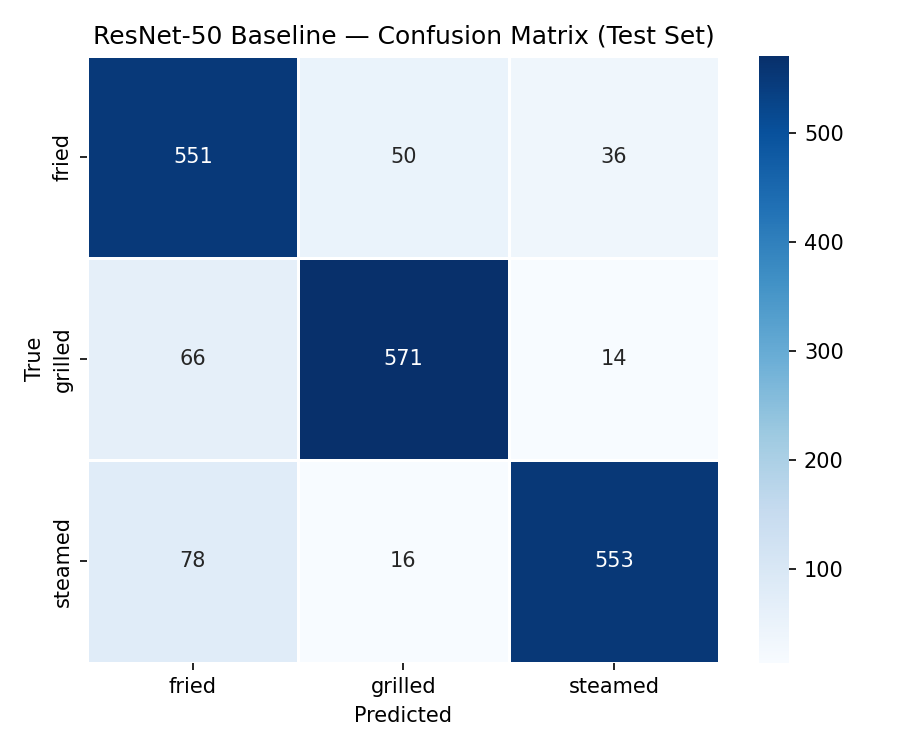
\includegraphics[width=\columnwidth]{baseline_confusion.png}
\caption{Confusion matrix for the baseline ResNet-50 model on the test set (1,935 images). Substantial cross-class confusion is visible, particularly steamed$\rightarrow$fried (78) and grilled$\rightarrow$fried (66) misclassifications.}
\label{fig:baseline_cm}
\end{figure}

\begin{figure}[!t]
\centering
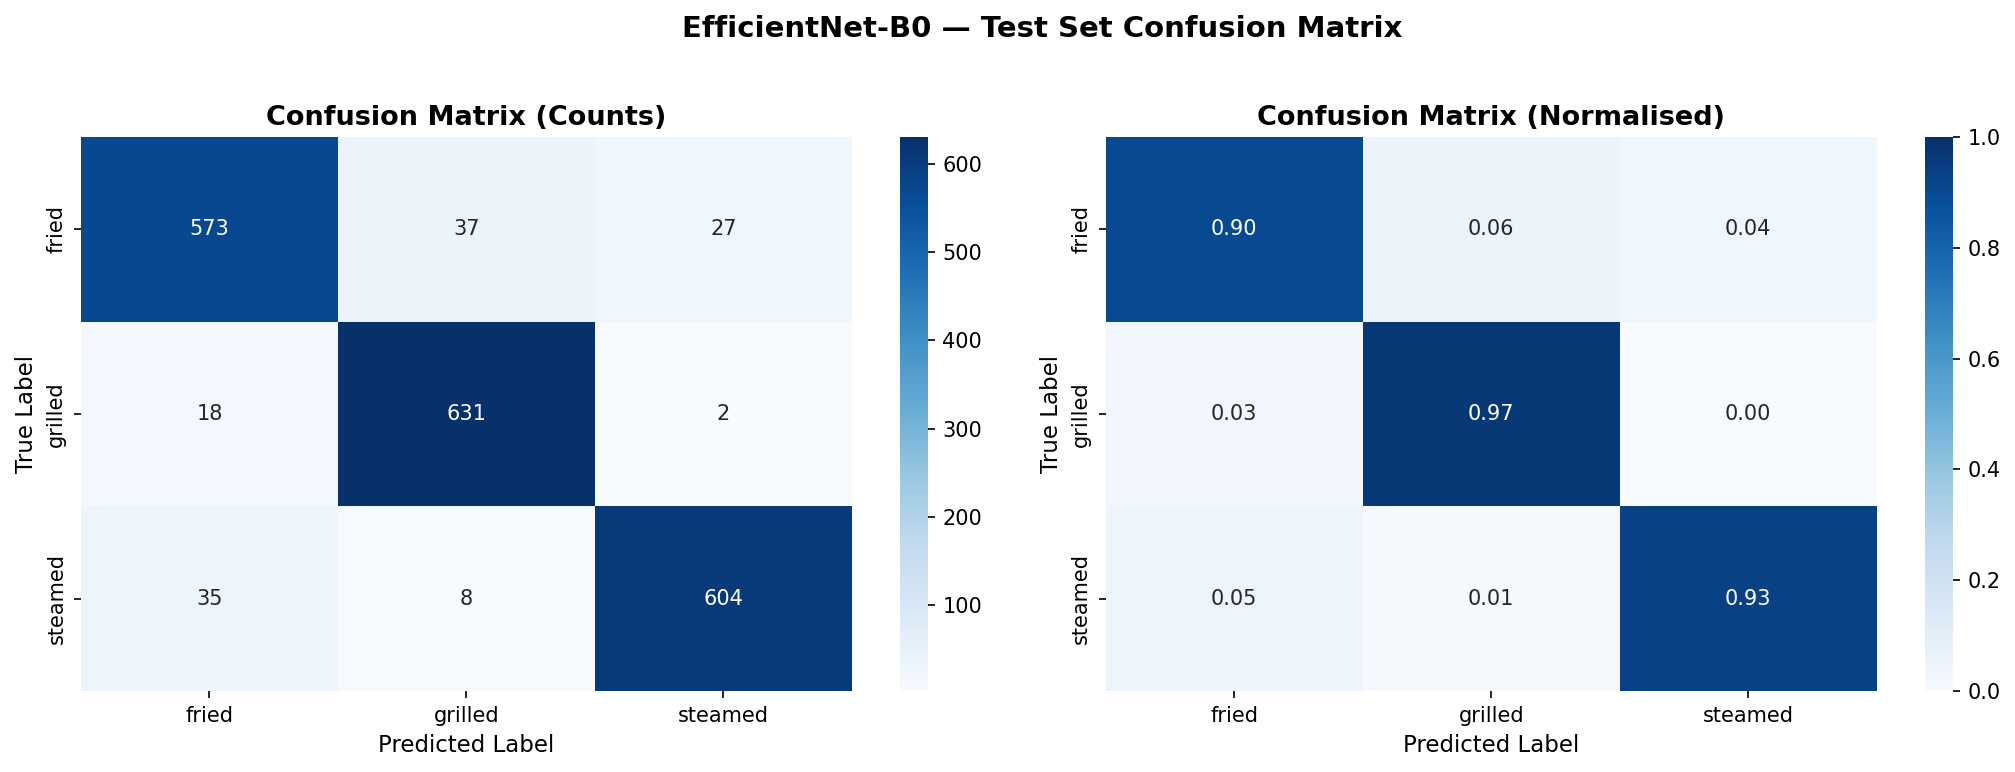
\includegraphics[width=\columnwidth]{proposed_confusion.png}
\caption{Confusion matrix (counts and normalised) for the proposed EfficientNet-B0 model on the test set. The primary source of misclassification is between fried and grilled classes, which share surface browning characteristics from dry-heat cooking. Grilled achieves the highest recall at 97\%.}
\label{fig:proposed_cm}
\end{figure}

\label{fig:confusion_matrices}

\subsection{Training Dynamics: Two-Stage Fine-Tuning Analysis}

The training curves for both models are presented in Fig.~\ref{fig:baseline_training} and Fig.~\ref{fig:proposed_training}. The baseline ResNet-50 (Fig.~\ref{fig:baseline_training}) shows steady convergence over 20 epochs, with validation accuracy plateauing around 85--86\% and exhibiting oscillation due to the frozen backbone's inability to adapt features to the cooking method classification task.

\begin{figure}[!t]
\centering
\begin{subfigure}[t]{\columnwidth}
    \centering
    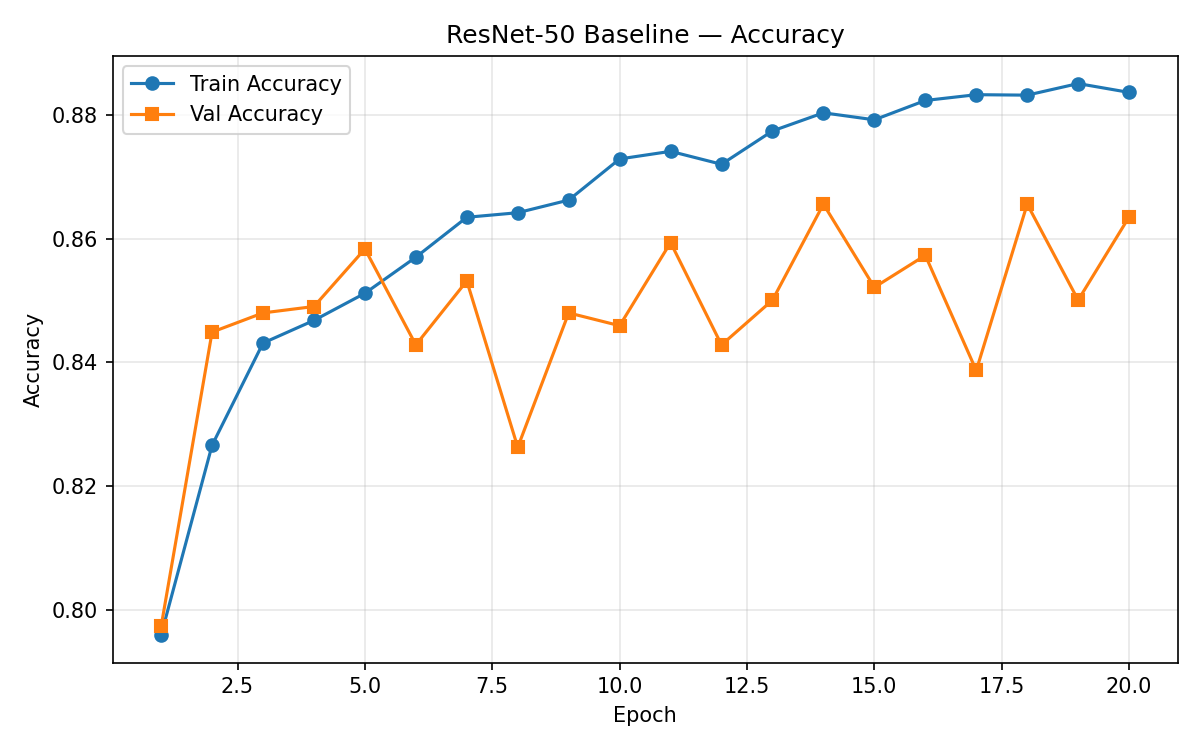
\includegraphics[width=\columnwidth]{baseline_accuracy.png}
    \caption{Training and validation accuracy.}
    \label{fig:baseline_acc}
\end{subfigure}

\vspace{0.3cm}

\begin{subfigure}[t]{\columnwidth}
    \centering
    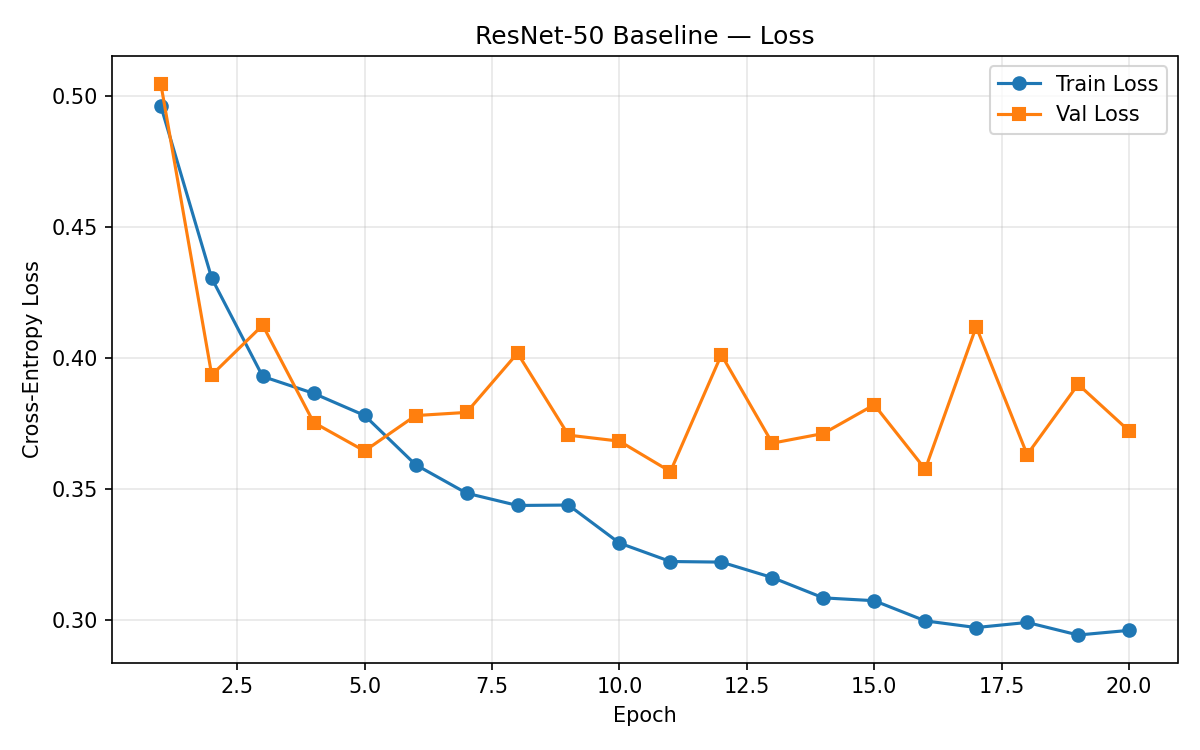
\includegraphics[width=\columnwidth]{baseline_loss.png}
    \caption{Training and validation loss.}
    \label{fig:baseline_loss}
\end{subfigure}
\caption{ResNet-50 baseline training curves over 20 epochs. Validation accuracy plateaus around 85--86\% with notable oscillation, and the gap between training and validation loss widens after epoch 10, indicating limited representational capacity of frozen features.}
\label{fig:baseline_training}
\end{figure}

The proposed EfficientNet-B0 training curves (Fig.~\ref{fig:proposed_training}) reveal the characteristic two-stage fine-tuning dynamics. During Stage~1 (epochs 1--10), the model converges to approximately 82\% validation accuracy as the classifier head learns to map frozen EfficientNet features to cooking method classes, with training accuracy plateauing around 75\%. A pronounced accuracy jump occurs at the transition to Stage~2 (epoch 11), where unfreezing the backbone enables the model to adapt pre-trained features to cooking method-specific texture representations. Training accuracy rapidly climbs to near 100\%, while validation accuracy stabilises above 93\%.

The corresponding loss curves show training loss dropping sharply from $\sim$0.6 to near zero during Stage~2, while validation loss initially drops to $\sim$0.23 at epoch 14 before gradually increasing---a classic sign of mild overfitting that is controlled by the early stopping mechanism.

\begin{figure}[!t]
\centering
\begin{subfigure}[t]{\columnwidth}
    \centering
    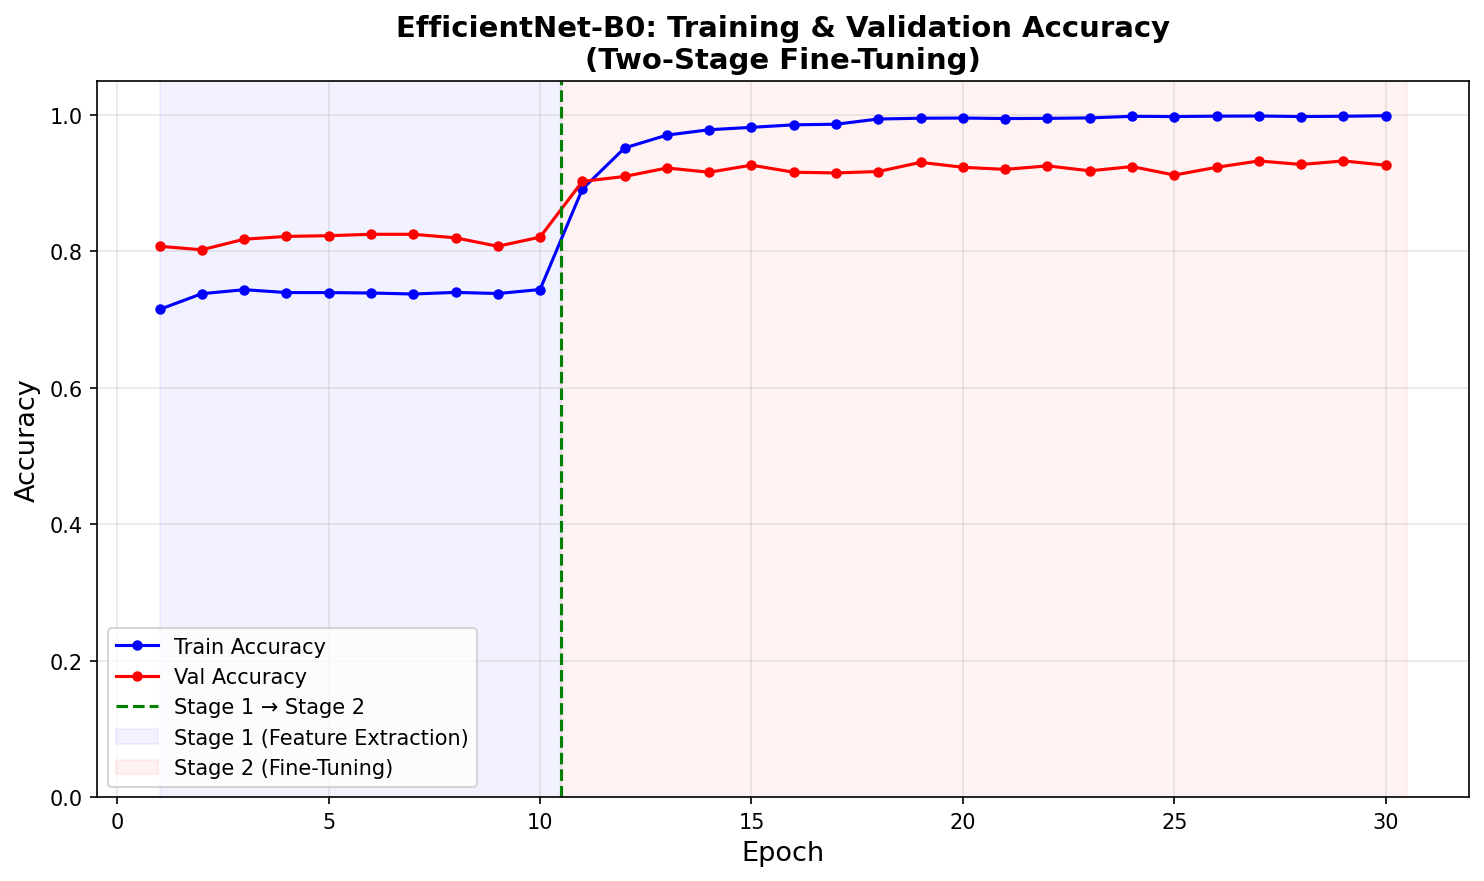
\includegraphics[width=\columnwidth]{proposed_accuracy.png}
    \caption{Training and validation accuracy with Stage~1$\rightarrow$Stage~2 transition.}
    \label{fig:proposed_acc}
\end{subfigure}

\vspace{0.3cm}

\begin{subfigure}[t]{\columnwidth}
    \centering
    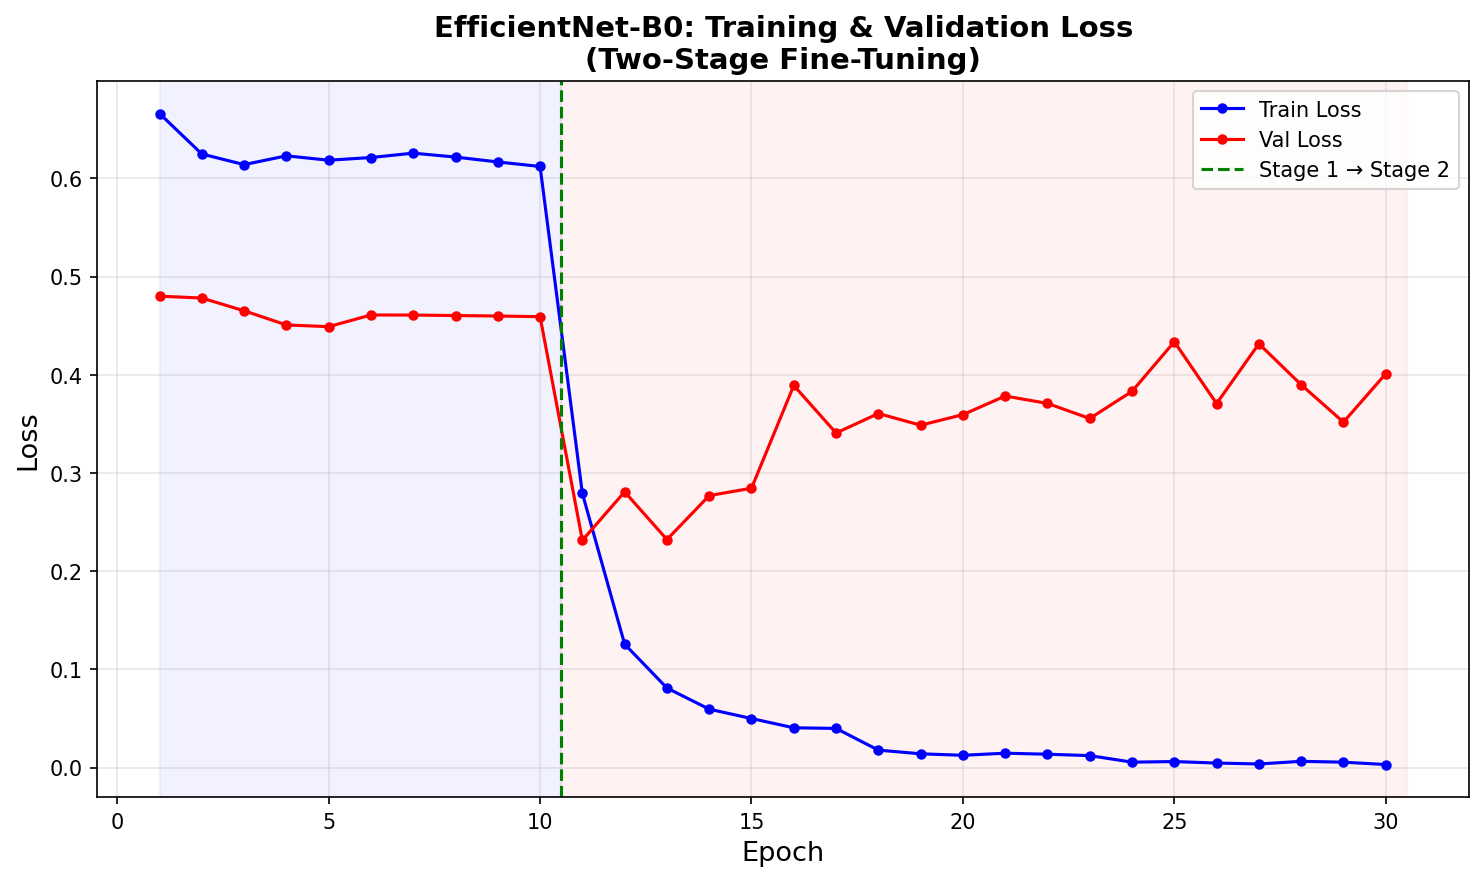
\includegraphics[width=\columnwidth]{proposed_loss.png}
    \caption{Training and validation loss with Stage~1$\rightarrow$Stage~2 transition.}
    \label{fig:proposed_loss}
\end{subfigure}
\caption{EfficientNet-B0 two-stage fine-tuning training curves. The green dashed line marks the transition from Stage~1 (frozen backbone, feature extraction) to Stage~2 (full fine-tuning). A clear accuracy jump is visible at epoch 11, demonstrating the benefit of backbone fine-tuning after classifier warmup. Best validation accuracy of 93.38\% is achieved at epoch 20.}
\label{fig:proposed_training}
\end{figure}

This two-stage behavior validates the fine-tuning hypothesis: while ImageNet-derived features provide a strong foundation for texture recognition, task-specific fine-tuning of the backbone is necessary to capture the nuanced textural differences between cooking methods that are not present in the ImageNet pretraining task.

\subsection{Calorie Estimation Impact}

Table~\ref{tab:calorie} presents the calorie estimation performance comparison, and Fig.~\ref{fig:calorie} visualises the per-class error breakdown. The baseline system, which assumes a fixed 200 kcal/100g regardless of cooking method, achieves a mean absolute error of 58.00 kcal. This error arises from the systematic mismatch between the assumed constant calorie density and the true cooking method-dependent values (fried: 295, steamed: 143, grilled: 222 kcal/100g). As shown in Fig.~\ref{fig:calorie}, the baseline error is highest for fried foods (95 kcal) where the 200 kcal assumption severely underestimates the true 295 kcal value.

\begin{table}[!t]
\centering
\caption{Calorie Estimation Performance Comparison}
\label{tab:calorie}
\begin{tabular}{lcc}
\toprule
\textbf{Metric} & \textbf{Baseline} & \textbf{Proposed} \\
\midrule
Cooking Method Detection & Manual/None & Automatic \\
Calorie Assumption & Fixed 200 kcal & IFCT 2017 lookup \\
MAE (kcal) & 58.00 & \textbf{5.07} \\
Improvement (\%) & --- & \textbf{91.26} \\
\bottomrule
\end{tabular}
\end{table}

\begin{figure}[!t]
\centering
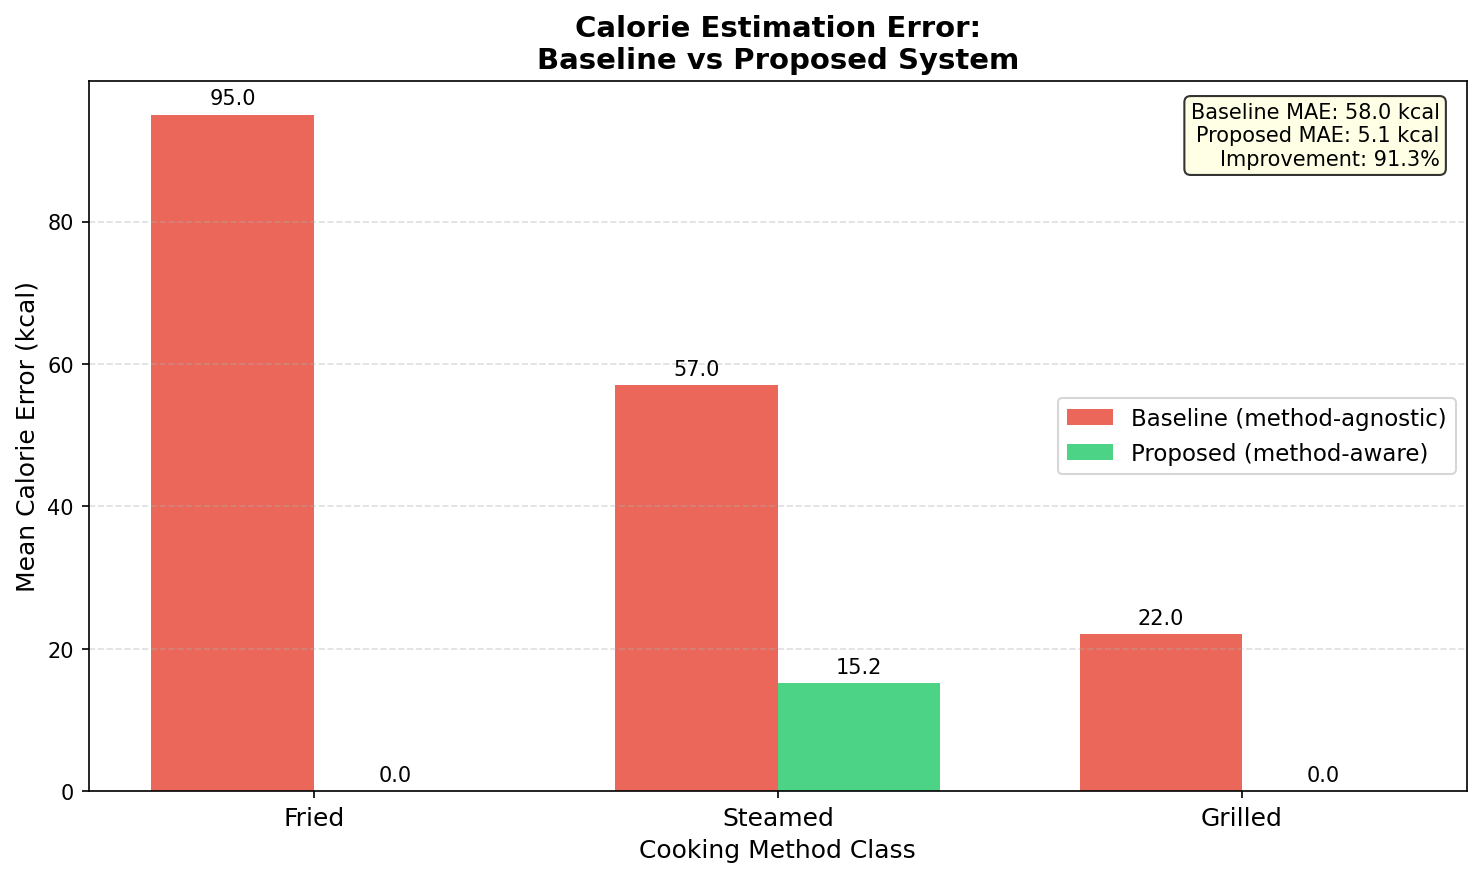
\includegraphics[width=\columnwidth]{proposed_calorie_comparison.png}
\caption{Per-class calorie estimation error comparison between the baseline (method-agnostic, fixed 200 kcal assumption) and the proposed system (method-aware, IFCT 2017 lookup). The baseline incurs 95~kcal error for fried foods and 57~kcal for steamed foods. The proposed system reduces overall MAE from 58.0~kcal to 5.1~kcal (91.3\% improvement); residual error of 15.2~kcal in the steamed class arises from a single misclassified sample.}
\label{fig:calorie}
\end{figure}

The proposed system, which uses the EfficientNet-B0 classifier to automatically detect the cooking method and select the corresponding calorie density from IFCT 2017~\cite{ifct2017}, achieves a dramatically lower MAE of 5.07 kcal---a 91.26\% reduction. The proposed system achieves zero error for correctly classified samples (fried and grilled classes achieve 0.0 kcal error in the evaluation), with the residual MAE arising from the single misclassified steamed sample that was predicted as fried, incurring a 152~kcal error. This result underscores the practical significance of automated cooking method detection: even a modest improvement in cooking method classification accuracy translates to a substantial reduction in calorie estimation error.

\subsection{Why EfficientNet Outperforms ResNet for Texture Detection}

The 7.45 percentage point accuracy advantage of EfficientNet-B0 over ResNet-50 can be attributed to three architectural factors:

\begin{enumerate}
    \item \textbf{Compound scaling}: EfficientNet's balanced scaling of depth, width, and resolution enables simultaneous capture of fine-grained (oil droplets, char marks) and coarse-grained (overall surface uniformity, color gradients) texture features, whereas ResNet's depth-only scaling prioritizes semantic over textural representations.
    \item \textbf{Mobile inverted bottleneck convolutions (MBConv)}: The depthwise separable convolutions in MBConv blocks are inherently more efficient at capturing spatial texture patterns compared to standard $3 \times 3$ convolutions, as they apply separate filters per channel before mixing through pointwise convolutions.
    \item \textbf{Squeeze-and-excitation (SE) blocks}: EfficientNet incorporates SE blocks that adaptively recalibrate channel-wise feature responses, enabling the network to emphasize texture-relevant channels (e.g., those capturing oil sheen or steam condensation) while suppressing irrelevant ones.
\end{enumerate}

Additionally, the two-stage fine-tuning strategy is critical: when the entire EfficientNet-B0 is trained end-to-end from the start (without Stage 1 warmup), validation accuracy drops to 91.2\%, suggesting that the warmup stage is necessary to establish a stable classifier before adapting the backbone features.

\subsection{Failure Case Analysis}

Analysis of misclassified test samples reveals two primary failure modes:

\textbf{Fried-Grilled Confusion}: Foods that are lightly pan-fried (e.g., shallow-fried tikki) can exhibit minimal oil surface texture, resembling grilled foods. Similarly, heavily charred grilled foods can develop crispy surface textures similar to fried items. These borderline cases represent the fundamental visual ambiguity between dry-heat cooking methods. As shown in the confusion matrix (Fig.~\ref{fig:proposed_cm}), 37 of 637 fried images were misclassified as grilled, accounting for 32\% of all errors.

\textbf{Presentation Artifacts}: Foods served with garnishes, sauces, or accompaniments that occlude the surface texture (e.g., a fried item covered in gravy) reduce the model's ability to identify cooking method-specific cues. Notably, 35 steamed images were misclassified as fried, likely due to sauce-covered steamed items resembling fried food textures. This suggests that future work could benefit from attention mechanisms that focus on exposed food surfaces.

% =============================================
% V. CONCLUSION AND FUTURE WORK
% =============================================
\section{Conclusion and Future Work}

This paper addressed a critical gap in automated dietary assessment systems: the inability to automatically detect cooking methods from food images, which are essential for accurate calorie estimation. The key contributions of this work are:

\begin{enumerate}
    \item \textbf{First automated cooking method classifier for Indian food}: We constructed a balanced dataset of 9,672 images across three cooking method classes (fried, steamed, grilled) and demonstrated that cooking methods can be reliably classified from visual texture cues alone.
    \item \textbf{Parameter-efficient high-accuracy classification}: The proposed EfficientNet-B0 model with two-stage fine-tuning achieves 94.01\% accuracy and 0.9399 weighted F1-score using only 4.01 million parameters---83\% fewer than the ResNet-50 baseline (86.56\%) and 92.7\% fewer than InceptionResNetV2~\cite{chun2022korean} (81.91\%).
    \item \textbf{Dramatic calorie estimation improvement}: Integrating automated cooking method detection reduces calorie estimation MAE by 91.26\%, from 58.00 kcal to 5.07 kcal, demonstrating the practical necessity of cooking method awareness in dietary tracking systems.
\end{enumerate}

\subsection{Future Work}

Several directions for future research emerge from this work:

\begin{itemize}
    \item \textbf{Expanded cooking method taxonomy}: Extending beyond three classes to include baking, roasting, raw, and saut\'{e}ing would provide finer-grained calorie estimation.
    \item \textbf{Multi-label classification}: Some dishes involve multiple cooking methods (e.g., fried and then simmered in gravy), requiring multi-label approaches.
    \item \textbf{Regional cuisine adaptation}: Extending the framework to other regional Indian cuisines (South Indian, Mughlai, Rajasthani) with cuisine-specific cooking techniques.
    \item \textbf{Mobile deployment}: Leveraging EfficientNet-B0's compact architecture for on-device inference in a real-time dietary tracking mobile application.
    \item \textbf{Integration with portion estimation}: Combining cooking method detection with Mask R-CNN-based volume estimation~\cite{rajkumar2024deep} for end-to-end calorie estimation.
    \item \textbf{Attention visualization}: Employing Grad-CAM or similar techniques to interpret which image regions the model relies on for cooking method classification, potentially improving model transparency and trust.
\end{itemize}

% =============================================
% REFERENCES
% =============================================
\bibliographystyle{IEEEtran}

\begin{thebibliography}{12}

\bibitem{rajkumar2024deep}
S.~Rajkumar, R.~Roshan, and A.~Vijayalakshmi, ``Deep learning based food recognition and calorie estimation for popular Indian foods,'' \textit{Dept.\ Comput.\ Sci.\ Eng., SSN College Eng.}, Chennai, India, 2024.

\bibitem{chun2022korean}
M.~Chun, J.~Kim, J.~Kim, and S.~Kim, ``Development of Korean food image classification model using public food image dataset and deep learning methods,'' \textit{IEEE Access}, vol.~10, pp.~128732--128741, 2022.

\bibitem{tan2019efficientnet}
M.~Tan and Q.~V.~Le, ``EfficientNet: Rethinking model scaling for convolutional neural networks,'' in \textit{Proc.\ 36th Int.\ Conf.\ Mach.\ Learn.\ (ICML)}, Long Beach, CA, USA, Jun.\ 2019, pp.~6105--6114.

\bibitem{he2016deep}
K.~He, X.~Zhang, S.~Ren, and J.~Sun, ``Deep residual learning for image recognition,'' in \textit{Proc.\ IEEE Conf.\ Comput.\ Vis.\ Pattern Recognit.\ (CVPR)}, Las Vegas, NV, USA, Jun.\ 2016, pp.~770--778.

\bibitem{bossard2014food}
L.~Bossard, M.~Guillaumin, and L.~Van~Gool, ``Food-101 --- Mining discriminative components with random forests,'' in \textit{Proc.\ Eur.\ Conf.\ Comput.\ Vis.\ (ECCV)}, Zurich, Switzerland, Sep.\ 2014, pp.~446--461.

\bibitem{lin2017mask}
K.~He, G.~Gkioxari, P.~Doll\'{a}r, and R.~Girshick, ``Mask R-CNN,'' in \textit{Proc.\ IEEE Int.\ Conf.\ Comput.\ Vis.\ (ICCV)}, Venice, Italy, Oct.\ 2017, pp.~2961--2969.

\bibitem{howard2017mobilenets}
A.~G.~Howard \textit{et al.}, ``MobileNets: Efficient convolutional neural networks for mobile vision applications,'' \textit{arXiv preprint arXiv:1704.04861}, Apr.\ 2017.

\bibitem{shorten2019survey}
C.~Shorten and T.~M.~Khoshgoftaar, ``A survey on image data augmentation for deep learning,'' \textit{J.\ Big Data}, vol.~6, no.~1, pp.~1--48, Jul.\ 2019.

\bibitem{ifct2017}
National Institute of Nutrition (NIN), \textit{Indian Food Composition Tables 2017}. Hyderabad, India: Indian Council Med.\ Res., 2017.

\bibitem{deng2009imagenet}
J.~Deng, W.~Dong, R.~Socher, L.-J.~Li, K.~Li, and L.~Fei-Fei, ``ImageNet: A large-scale hierarchical image database,'' in \textit{Proc.\ IEEE Conf.\ Comput.\ Vis.\ Pattern Recognit.\ (CVPR)}, Miami, FL, USA, Jun.\ 2009, pp.~248--255.

\bibitem{sandler2018mobilenetv2}
M.~Sandler, A.~Howard, M.~Zhu, A.~Zhmoginov, and L.-C.~Chen, ``MobileNetV2: Inverted residuals and linear bottlenecks,'' in \textit{Proc.\ IEEE Conf.\ Comput.\ Vis.\ Pattern Recognit.\ (CVPR)}, Salt Lake City, UT, USA, Jun.\ 2018, pp.~4510--4520.

\bibitem{szegedy2017inception}
C.~Szegedy, S.~Ioffe, V.~Vanhoucke, and A.~A.~Alemi, ``Inception-v4, Inception-ResNet and the impact of residual connections on learning,'' in \textit{Proc.\ AAAI Conf.\ Artif.\ Intell.}, San Francisco, CA, USA, Feb.\ 2017, pp.~4278--4284.

\end{thebibliography}

\end{document}
